\documentclass[11pt,a4paper]{article}

% Packages
\usepackage[utf8]{inputenc}
\usepackage[spanish, es-tabla]{babel}
\usepackage{amsmath}
\usepackage{amssymb}
\usepackage{upgreek}
\usepackage{accents}
\usepackage[shortlabels]{enumitem}
\usepackage{graphicx}
\usepackage{parskip}
\usepackage{array}
\usepackage[table]{xcolor}
\usepackage{tikz}		% Tener números dentro de cículos (\circled).
\usepackage{mdwlist} % Cambiar los índices en enumerate.
\usepackage{xfrac}		% Fracciones en diagonal (\sfrac).
\usepackage{lmodern} % Eliminar warning de Font shape.
\usepackage{mathtools}
\usepackage{xcolor}

% Definición de circled.
\newcommand*{\circled}[2][]{\tikz[baseline=(C.base)]{
	\node[inner sep=0pt] (C) {\vphantom{1g}#2};
	\node[draw, circle, inner sep=1pt, yshift=1pt]
		at (C.center) {\vphantom{1g}};}}
		
\newcolumntype{P}[1]{>{\centering\arraybackslash}p{#1}}
\newcolumntype{M}[1]{>{\centering\arraybackslash}m{#1}}
		
% Default fixed font does not support bold face
\DeclareFixedFont{\ttb}{T1}{txtt}{bx}{n}{12} % for bold
\DeclareFixedFont{\ttm}{T1}{txtt}{m}{n}{12}  % for normal

% Custom colors
\usepackage{color}
\definecolor{deepblue}{rgb}{0,0,0.5}
\definecolor{deepred}{rgb}{0.6,0,0}
\definecolor{deepgreen}{rgb}{0,0.5,0}

\usepackage{listings}

% Python style for highlighting
\newcommand\pythonstyle{\lstset{
language=Python,
basicstyle=\tiny,
morekeywords={self},              			% Add keywords here
keywordstyle=\color{deepblue},
emph={MyClass,__init__},          			% Custom highlighting
emphstyle=\ttb\color{deepred},    		% Custom highlighting style
stringstyle=\color{deepgreen},
frame=tb,                         					% Any extra options here
showstringspaces=false,
}}

% Python environment
\lstnewenvironment{python}[1][]
{
\pythonstyle
\lstset{#1}
}
{}

% Python for external files
\newcommand\pythonexternal[2][]{{
\pythonstyle
\lstinputlisting[#1]{#2}}}

% Python for inline
\newcommand\pythoninline[1]{{\pythonstyle\lstinline!#1!}}

\begin{document}
\begin{titlepage}
\centering

\includegraphics[width=0.15\textwidth]{./UGR.png}\par\vspace{1cm}
{\scshape\LARGE Universidad de Granada \par}
\vspace{1cm}
\vspace{1.5cm}
{\huge\bfseries Ingeniería del Conocimiento\par}
\vspace{2cm}
{\LARGE\bfseries Protégé\par}
\vspace{2cm}
{\Large\itshape Pedro Ramos Suárez\par}
\vfill
Doble Grado de Ingeniería Informática y Matemáticas
\vfill
{\large \today\par}
\end{titlepage}

\newpage

\section*{Ontología}

La ontología utilizada es:
\begin{center}
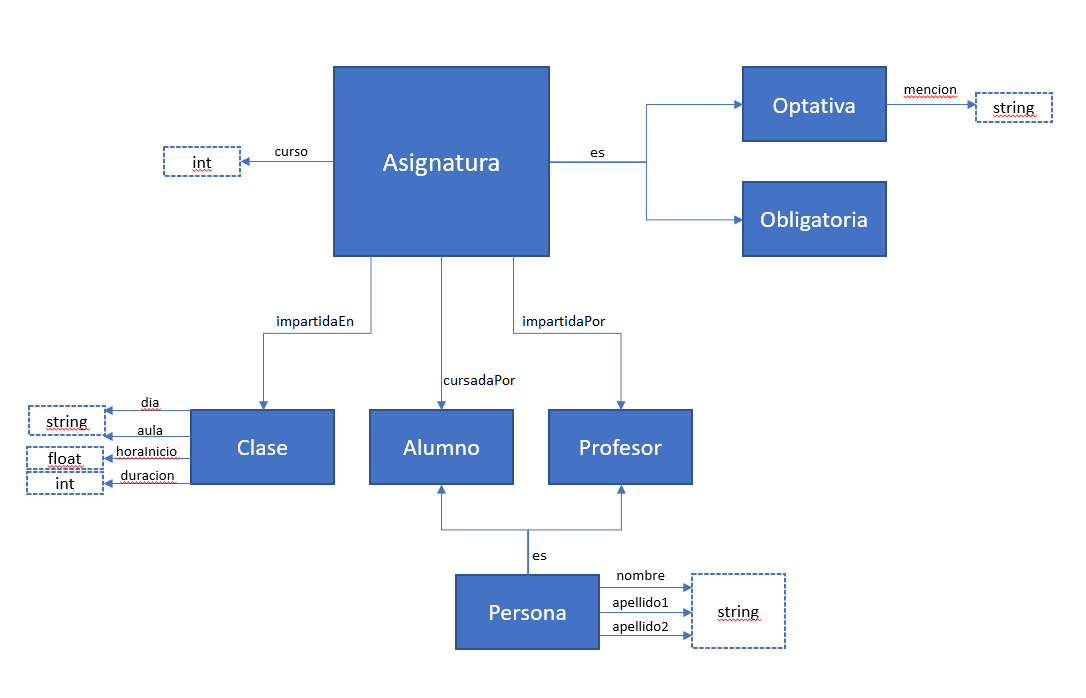
\includegraphics[width=1\textwidth]{./ontonlogia.PNG}\par\vspace{1cm}
\end{center}

Donde:
\begin{itemize}
\item Asignatura representa una asignatura. Puede ser de dos tipos:
\begin{itemize}
\item Optativa, que son las asignaturas de la mención, por lo que tiene la propiedad mencion, que es un array que puede ser ``Computación y Sistemas Inteligentes'', ``Ingeniería del Software'', ``Ingeniería del Computadores'', ``Sistemas de Información'' ó ``Tecnologías de la información''.
\item Obligatoria, siempre que no sea optativa. 
\end{itemize}
Además, todas las asignaturas tiene la propiedad curso, que es un entero entre 1 y 4 que indica el curso en el que se imparte dicha asignatura.
\item Clase, que representa cuando y donde se imparte una asignatura. Tiene de propiedades:
\begin{itemize}
\item dia, que es el día de la semana en el que se imparte. Puede ser ``Lunes'', ``Martes'', ``Miércoles'', ``Jueves'' o ``Viernes''.
\item aula, que es el nombre del aula en la que se imparte. Es un String con cualquier formato.
\item horaInicio, que indica la hora a la que comienza la clave. Es un float entre 0 y 24, por lo que, por ejemplo, las 16:00 sería 16.0f, y 16:30 sería 16.5f.
\item duracion, que indica la duración de la clase en minutos. Es un entero.
\end{itemize}
\item Persona, que representa a una persona. Puede ser de dos tipos:
\begin{itemize}
\item Alumno, representa a un alumno.
\item Profesor, representa a un profesor.
\end{itemize} 
Sus atributos son:
\begin{itemize}
\item nombre, es un string que contiene el nombre de la persona.
\item apellido1, es un es string que contiene el primer apellido de la persona.
\item apellido2, es un es string que contiene el segundo apellido de la persona.
\end{itemize}
\end{itemize}

\section*{Restricciones de los dominios}

Los atributos con dominios restringidos son:
\begin{itemize}
\item Asignatura.curso: Los posibles cursos son 1, 2, 3 o 4, así que lo restringimos a:
\begin{lstlisting}[basicstyle=\scriptsize]
{"1"^^xsd:int , "2"^^xsd:int , "3"^^xsd:int , "4"^^xsd:int}
\end{lstlisting}
\item Optativa.mencion: Para restringirlo a las posibles menciones usamos:
\begin{lstlisting}[basicstyle=\scriptsize]
{"Computacion y Sistemas Inteligentes"^^xsd:string ,
"Ingenieria de Computadores"^^xsd:string ,
"Ingenieria del Software"^^xsd:string,
"Sistemas de Informacion"^^xsd:string ,
"Tecnologias de la Informacion"^^xsd:string}
\end{lstlisting}
\item Clase.dia: Para restringirlo a los posibles días de la semana usamos:
\begin{lstlisting}[basicstyle=\scriptsize]
{"Jueves"^^xsd:string , "Lunes"^^xsd:string ,
"Martes"^^xsd:string, "Miercoles"^^xsd:string ,
"Viernes"^^xsd:string}
\end{lstlisting}
\item Clase.horaInicio: Tiene que ser un float en [0, 24[, ya que son todas las horas del día, por lo que lo restringimos:
\begin{lstlisting}[basicstyle=\scriptsize]
xsd:float[> 0.0f , < 24.0f]
\end{lstlisting}
\end{itemize}

\section*{Axioma}

Debido a que no tenemos ningún axioma, vamos a añadir uno para que infiera información por este axioma, el cual va a ser que toda asignatura que sea optativa es de tercero. Aunque este axioma no es cierto en la realidad, ya que hay optativas en cuarto, nos sirve como ejemplo para inferir valores. Para ello añadimos:
\begin{lstlisting}[basicstyle=\scriptsize]
Optativa SubClassOf curso value "3"^^xsd:int
\end{lstlisting}

\section*{Ejemplos de inferencias}

\subsection*{Inferencia de jerarquía}

\begin{center}
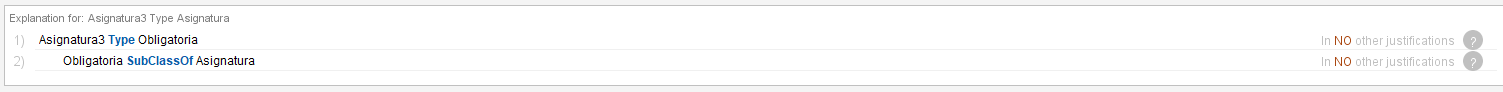
\includegraphics[width=1\textwidth]{./jerarquia.PNG}\par\vspace{1cm}
\end{center}

En la imagen de arriba podemos observar como deduce que Asignatura3 es una asignatura ya que Obligatoria es una subclase de Asignatura.

\subsubsection*{Inferencia de clase}

\begin{center}
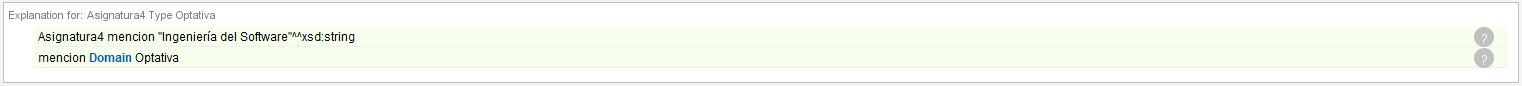
\includegraphics[width=1\textwidth]{./clase.PNG}\par\vspace{1cm}
\end{center}

En la imagen de arriba podemos observar como deduce que Asignatura4 es una Optativa al tener un valor en el campo mencion, cuyo dominio es la clase Optativa.

\subsubsection*{Inferencia de valor}

\begin{center}
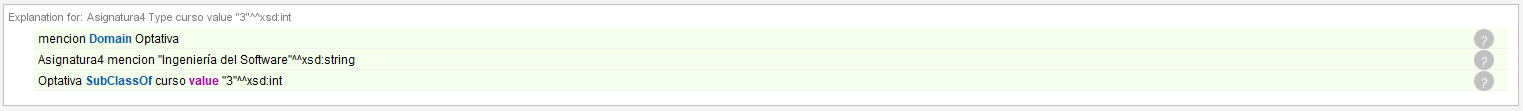
\includegraphics[width=1\textwidth]{./valor.PNG}\par\vspace{1cm}
\end{center}

En la imagen de arriba podemos observar como deduce que Asignatura4 es de tercero por ser una Optativa, usando el axioma definido previamente.

\end{document}